\documentclass[10pt,twocolumn,twoside]{IEEEtran}

\usepackage{afterpage}
\usepackage{bold-extra}
\usepackage{color}
\usepackage{float}
\usepackage{graphicx}
\usepackage{listings}
\usepackage{subfigure}

%%%%%%%%%%%%%%%
%%% Colours %%%
%%%%%%%%%%%%%%%

\definecolor{darkgreen}{rgb}{0, 0.6, 0}
\definecolor{lightgrey}{gray}{0.9}

%%%%%%%%%%%
% Figures %
%%%%%%%%%%%

% Define shorter ways to include individual images
\newcommand{\stufig}[4]						% images with default placement
{
	\begin{figure}
	\begin{center}
		\includegraphics[#1]{#2}
		\caption{#3}
		\label{#4}
	\end{center}
	\end{figure}
}

\newcommand{\stufigex}[5]					% images with specified placement
{
	\begin{figure}[#5]
	\begin{center}
		\includegraphics[#1]{#2}
		\caption{#3}
		\label{#4}
	\end{center}
	\end{figure}
}

\newcommand{\stufigexx}[5]				% full-width images with specified placement
{
	\begin{figure*}[#5]
	\begin{center}
		\includegraphics[#1]{#2}
		\caption{#3}
		\label{#4}
	\end{center}
	\end{figure*}
}

% Define the stusubfig environment
\newenvironment{stusubfig}[1]
{
	\begin{figure*}[#1]
	\begin{center}
}
{
	\end{center}
	\end{figure*}
}

%%%%%%%%%%%%%%%%%
% Code Listings %
%%%%%%%%%%%%%%%%%

% Create a new type of float (called a stulisting) for listings
\floatstyle{ruled}
\newfloat{stulisting}{thp}{lop}
\floatname{stulisting}{Listing}

% Setup before using the listings package
\renewcommand{\lstlistingname}{\textbf{Listing}}
\def\thelstlisting{\textbf{\arabic{lstlisting}}}

\lstdefinelanguage{Pseudocode}{
morekeywords={and,assert,break,case,continue,default,down,each,else,for,function,if,not,null,or,rangeswitch,ref,return,switch,then,this,throw,to,up,var,while},
sensitive=true,
morecomment=[l]{//},
morecomment=[s]{/*}{*/}
}

\lstdefinestyle{Default}{
abovecaptionskip=0.5cm,
basicstyle=\scriptsize\ttfamily,
belowcaptionskip=0.5cm,
belowskip=0.5cm,
columns=fixed,
%commentstyle=\color{darkgreen},
commentstyle=\textit, % changed from the thesis (green text looks unprofessional in a journal paper)
language=Pseudocode,
%numbers=left,
numbers=none, % changed from the thesis (line numbers are less relevant here)
numbersep=5pt,
numberstyle=\tiny,
mathescape=true,
showstringspaces=false,
stepnumber=1,
tabsize=4
}

\lstdefinestyle{Snippet}{
abovecaptionskip=0.5cm,
aboveskip=0.5cm,
basicstyle=\small\ttfamily,
belowcaptionskip=0.5cm,
belowskip=0.5cm,
columns=fixed,
commentstyle=\color{darkgreen},
frame=lines,
keywordstyle=\small\bfseries,
language=Pseudocode,
numbers=none,
mathescape=true,
showstringspaces=false,
stepnumber=1,
tabsize=4
}

% For C++ function prototypes
\lstdefinestyle{Prototype}{
abovecaptionskip=0.5cm,
basicstyle=\small\ttfamily,
belowcaptionskip=0.5cm,
belowskip=0.5cm,
columns=fixed,
commentstyle=\color{darkgreen},
language=C++,
numbers=none,
mathescape=true,
showstringspaces=false,
stepnumber=1,
tabsize=4
}

%%%%%%%%%%%%%%%%%%%%
% Special Commands %
%%%%%%%%%%%%%%%%%%%%

\newcommand{\svlis}{%
\mbox{\scriptsize S\hspace{-0.2mm}\footnotesize V\hspace{-0.2mm}%
\normalsize L\hspace{0.1mm}\footnotesize I\hspace{0.2mm}\scriptsize S\ }}

%%%%%%%%%%%%%%%%%
% Main Document %
%%%%%%%%%%%%%%%%%

\begin{document}

\title{Automatic Multi-Feature Identification in Abdominal CT Scans}

\author{Stuart~Golodetz, Irina~Voiculescu and Stephen~Cameron%
\thanks{S.~Golodetz was with the University of Oxford 2006--2011.}%
\thanks{I. Voiculescu and S. Cameron are with the University of Oxford.}}

\date{\today}

\markboth{IEEE Transactions on Image Processing, Vol.~?, No.~?,~?~2014}%
{Golodetz \MakeLowercase{\textit{et al.}}: Automatic Multi-Feature Identification in Abdominal CT Scans}

\IEEEpubid{0000--0000/00\$00.00~\copyright~2014 IEEE}

\maketitle

\begin{abstract}
\noindent The automatic identification of features (e.g.~bone structures and organs) in medical images is an important precursor to a number of tasks, including 3D visualisation, volume estimation and landmark-based registration. However, automatic techniques in the literature have tended to focus on the identification of individual features, with relatively few attempts being made to identify multiple features within a single framework due to the challenges involved in identifying even individual features automatically and the fact that techniques often need to be quite specialised for each feature type. Despite this, we believe that it can often make sense to identify multiple features together, since correctly identifying some features can be of great help when identifying others. Bone structures in particular are especially helpful landmarks due to their rigidity, and our earlier work on ribs and spine identification showed that bone structures could be automatically identified in 2D abdominal CT scans using approaches based on \emph{image partition forests} (IPFs). In this paper, we extend this work to show that similar techniques can be used to identify bone structures in 3D, and present preliminary results showing that the identified structures can be used to guide the identification of other features such as the spinal canal, aorta and kidneys.
\end{abstract}

\begin{IEEEkeywords}
abdominal CT scans, feature identification, image partition forests
\end{IEEEkeywords}

\IEEEpeerreviewmaketitle

%#####################
\section{Introduction}
%#####################

TODO

\textbf{The organisation of this paper is as follows:} in \S\ref{sec:background}, we briefly revisit the image partition forest (IPF) data structure and our original work on 2D rib and spine identification; in \S\ref{sec:bone3d}, we present our approach to identifying bone structures in 3D abdominal CT scans; in \S\ref{sec:multi3d}, we show how the identified bone structures can guide identification of the spinal canal, aorta and kidneys; in \S\ref{sec:experiments}, we TODO; and in \S\ref{sec:discussion}, we evaluate the results of our experiments and examine ways in which our work could be taken forwards.

%#####################
\section{Background}
\label{sec:background}
%#####################

\subsection{Image Partition Forests}

TODO

%---
\stufigex{width=.85\linewidth}{ipfs-ctconcept.png}{An example partition forest for an abdominal CT scan. (TODO: Create a version of this with multiple features identified.)}{fig:ipfs-ctconcept}{htb}
%---

\subsection{2D Rib and Spine Identification}

TODO: \cite{gvccimi08,gvcispa09}

TODO: Limitations

%#########################################
\section{3D Bone Structure Identification}
\label{sec:bone3d}
%#########################################

\IEEEpubidadjcol

TODO

%########################################
\section{3D Multi-Feature Identification}
\label{sec:multi3d}
%########################################

TODO: \cite{golodetz11}

%######################
\section{Experiments}
\label{sec:experiments}
%######################

TODO

%#####################
\section{Discussion}
\label{sec:discussion}
%#####################

TODO

%#####################################
\section{Conclusions and Further Work}
\label{sec:conclusions}
%#####################################

TODO

%#########################
\section{Acknowledgements}
%#########################

We are profoundly grateful to Dr.\ Zoe Traill of the Churchill Hospital, Oxford, both for providing us with abdominal CT scans and for giving up her time to help us interpret them. We also gratefully acknowledge the support of the UK Engineering and Physical Sciences Research Council (EPSRC) in funding Stuart Golodetz's doctoral work via a Doctoral Training Account (DTA).

\clearpage

\bibliographystyle{alpha}
\bibliography{existingwork,mypapers}

\vspace{1cm}

\begin{IEEEbiography}[{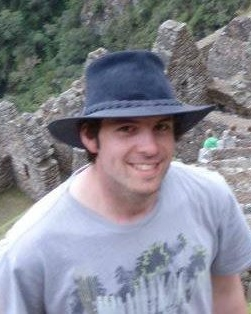
\includegraphics[width=1in,height=1.25in,clip,keepaspectratio]{pic_stuart.jpg}}]{Stuart Golodetz}
obtained his DPhil in Computer Science at Oxford University, working on 3D image segmentation and feature identification. He then spent two interesting years in industry, working in the areas of credit risk management, logic programming and software analytics. His areas of interest include medical image analysis, computer games development and the intricacies of different programming languages, especially C++. He was a session chair for the 6th International Symposium on Image and Signal Processing and Analysis, ISPA 2009. He is a member of the Association of C and C++ Users (ACCU) and has written a number of articles for their magazines.
\end{IEEEbiography}

\begin{IEEEbiography}[{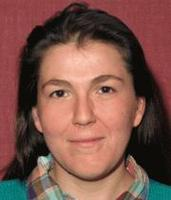
\includegraphics[width=1in,height=1.25in,clip,keepaspectratio]{pic_irina.jpg}}]{Irina Voiculescu}
is a Lecturer in Computer Science at the University of Oxford. She obtained a PhD at the University of Bath, for research in Constructive Solid Geometry. She contributed to the development of the geometric modelling software \svlis through the application of polynomial root finding methods. She works in the general area of geometric modelling, specifically focusing on the mathematics of curves and surfaces, interval arithmetic, molecular modelling and medical image analysis. She is a Fellow of the UK Geometric Modelling Society.
\end{IEEEbiography}

\begin{IEEEbiography}[{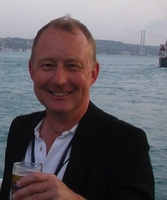
\includegraphics[width=1in,height=1.25in,clip,keepaspectratio]{pic_stephen.jpg}}]{Stephen Cameron}
obtained his PhD in Artificial Intelligence at Edinburgh University, working on the geometric modelling of robots and on collision detection. His general area of interest is in spatial reasoning, although this covers a wide range which includes the planning of tasks and motions for robot vehicles and manipulators, the use of geometric models, and the scheduling of group of flying or walking robots. He is a Reader in Computer Science at the University of Oxford. He is a member of the AISB, the IEEE Robotics and Automation Society, and the Geometric Modelling Society.
\end{IEEEbiography}

\end{document}
